% Bridges 2026 — Strukturvorschlag (kein Volltext)
% Okto-Computing / EABC-Brückenmanuskript
% Stand: 2026-07-07
% Kompilierbar als Gliederung; Inhalte als Platzhalter.

\documentclass[11pt,a4paper]{article}
\usepackage[utf8]{inputenc}
\usepackage[T1]{fontenc}
\usepackage{amsmath,amssymb}
\usepackage{booktabs}
\usepackage{graphicx}
\usepackage{hyperref}
\usepackage[most]{tcolorbox}

\newcommand{\evidence}[1]{\textnormal{[\,#1\,]}}
\newcommand{\placeholder}[1]{\textit{[#1]}}
\newcommand{\repo}[1]{\texttt{#1}}

\title{Okto-Computing Bridges:\\
  Quaternionic EABC Channels, Host Geometry, and Arithmetic Interference\\
  \large\textit{Bridges 2026 --- Structure Outline (not full manuscript)}}
\author{Thomas Hofbauer}
\date{2026-07-07}

\begin{document}
\maketitle

\begin{abstract}
\placeholder{1--2 Absätze: Vierkanal-Signatur $H(n)=(E,A,B,C)$, Hurwitz-/Oktonion-Lattice,
Dumas-Host-Komplementarität, illustrative Riemann-Interferenz und defensive Physik-Brücken.
Kein RH-Beweis, kein Collatz-Beweis, keine Physik-Identität.}
\end{abstract}

% ---------------------------------------------------------------------------
\begin{tcolorbox}[colback=gray!5,colframe=gray!60,title={Governance: Was ist bewiesen vs.\ illustriert vs.\ Analogie}]
\textbf{Legende:}
\evidence{A} = formal bewiesen (Lean / Satz);
\evidence{B} = reproduzierbare Diagnostik / Export, keine Theorem-Claim;
\evidence{C} = interpretive Analogie / Lesesprache / offene Hypothese.

\medskip
\begin{tabular}{@{}p{0.28\linewidth}p{0.65\linewidth}@{}}
\toprule
\textbf{Behauptungstyp} & \textbf{Beispiele in diesem Manuskript} \\
\midrule
Bewiesen \evidence{A} &
Dumas-Host-Komplementarität (E-048);
Collatz odd-core / $\nu_2$-Reduktion (Lean S1--S3);
Hurwitz-Sieb: keine ungeraden Primnormen auf $E_8$ in $[-5,5]^8$. \\
Illustriert \evidence{B} &
Riemann-Phasenkollaps-Plots (E-095);
fractional-weighted Kernel-Vergleich $\alpha{=}0$ vs.\ $\alpha{=}0.5$;
Kernbindungs-Residual-Export (E-092);
Collatz-Atlas-Diagnostik (kein Beweisclaim). \\
Analogie \evidence{C} &
Riemann-Nullstellen $\leftrightarrow$ bc-Achsen-Knoten;
Pauli-Bivektor-Symmetriebruch;
Kernbindung $R(A,Z)$ $\leftrightarrow$ $I_{\mathrm{EABC}}$;
Onsager/Dumas-Wirbel-Parallele. \\
\bottomrule
\end{tabular}

\medskip
\textbf{Nicht behaupten:}
RH-Beweis; Collatz-Vollbeweis; Caputo-Derivative für $\Phi_{R,\alpha}$;
physikalische Identität EABC $\equiv$ Nukleonen/QEC; discovery-taugliche
Prim-vs.-Komposit-Trennung ohne Präregistrierung.
\end{tcolorbox}
% ---------------------------------------------------------------------------

\tableofcontents
\newpage

% ===========================================================================
\section{Introduction and Conference Fit}
\label{sec:intro}

\subsection{Motivation: arithmetic geometry meets art/math bridges}
\placeholder{Bridges-Audience: visuelle und strukturelle Brücken zwischen Zahlentheorie,
Geometrie und physikalischer Lesesprache; Okto-Computing als 8D-Erweiterung der
quaternionischen EABC-Kanäle.}

\subsection{Contributions (tagged)}
\begin{enumerate}
  \item Energiedoku / EABC quaternion model \evidence{A}/\evidence{B}/\evidence{C}
  \item Dumas host vs.\ channel complementarity \evidence{A-T}/\evidence{B}
  \item Riemann interference diagnostic + fractional-weighted kernel \evidence{B}/\evidence{C}
  \item Symmetry breaking / bivector reading \evidence{C}
  \item Nuclear binding residual protocol \evidence{C} $\to$ \evidence{B}
  \item Collatz diagnostics appendix (no proof claims) \evidence{B}
\end{enumerate}

\subsection{Related work and repo map}
\placeholder{Verweis auf \repo{docs/paper-outline.md}, \repo{docs/theory/README.md}.}

% ===========================================================================
\section{Energiedoku and the EABC Quaternion Model}
\label{sec:eabc}

\subsection{Four-channel signature $H(n)=(E,A,B,C)$}
\evidence{A}/\evidence{B}
\placeholder{Additive Primfaktor-Kanäle; mod-12-Kegelschnitt-Lesart.}

\subsection{Quaternionic lift and octonionic extension sketch}
\evidence{C}
\placeholder{4D assoziativer Kern $\to$ 8D Oktonion-Slice; keine vollständige Okto-Theorie.}

\subsection{Floquet time ladder and shell resonance \#Energiedoku}
\evidence{B}/\evidence{C}
\placeholder{E-033--E-036; arithmetisch induzierte Schalen-Resonanz;
negative Evidenz E-034 (mean-cos auf $\Delta M$).}

\subsection{Reproducibility}
\repo{src/kepler_hurwitz/kepler_eabc_atlas.py},
\repo{docs/energiedoku_exports/}.

% ===========================================================================
\section{Dumas Host vs.\ Channel Geometry}
\label{sec:dumas}

\subsection{Dumas lemma and four-host complementarity}
\evidence{A-T}
\placeholder{Primvierling $(a,b,c,e)$; Gap kodiert Host; Lean E-048.}

\subsection{Double-cone lift, slice, and weight orbit}
\evidence{B}/\evidence{C}
\placeholder{H1--H11 Hypothesen-Kernel; Kepler-Kreis auf Kanal-Simplex.}

\subsection{Host slice vs.\ channel dynamics}
\placeholder{Host-Tripel vs.\ CEAB-Orbit; Gap-Rotor; keine physikalische Deduktion.}

\subsection{Reproducibility}
\repo{src/kepler_hurwitz/dumas_cone_orbit.py},
\repo{docs/theory/dumas_cone_orbit_model.md},
\repo{tests/test_dumas_cone_orbit.py}.

% ===========================================================================
\section{Riemann Interference at bc-Axis Nodes (E-095)}
\label{sec:riemann}

\subsection{Wave diagnostic $f(x)=\sum\cos(\gamma_n\ln x)$}
\evidence{C}
\placeholder{Explizite-Formel-Lesesprache; Odlyzko-Nullstellentabelle $N{=}150$.}

\subsection{Illustrative phase-collapse plots}
\evidence{B}
\placeholder{Fenster um $x{=}35$, $x{=}143$; Prim- vs.\ bc-Komposit-Markierungen.}

\subsection{Fractional-weighted kernel (NOT Caputo derivative)}
\evidence{B}/\evidence{C}
\begin{equation}
  \Phi_{R,\alpha}(x) = \sum_n \cos(\gamma_n \ln x)\, x^{-\alpha},
  \qquad \alpha \ge 0.
\end{equation}
\textbf{Terminologie:} \emph{fractional-weighted interference kernel} --- heuristischer
Speicherfilter, \textbf{keine} Implementierung einer Caputo-/Riemann-Liouville-Ableitung.
Für $\alpha{=}0$ gilt $\Phi_{R,0}=f$.

\subsection{PoC comparison $\alpha{=}0$ vs.\ $\alpha{=}0.5$}
\evidence{B}
\placeholder{Ehrliche Einordnung: $x^{-\alpha}$ skaliert Amplituden; verbessert
\emph{nicht} die absolute Trennung 35/31 oder 143/139; siehe
\repo{docs/manuscripts/bridges_2026_submission_notes.md}.}

\subsection{Reproducibility}
\repo{src/kepler_hurwitz/riemann_interference_diagnostics.py},
\repo{docs/theory/riemann_zero_interference_analogy.md},
\repo{tests/test_riemann_interference_diagnostics.py}.

% ===========================================================================
\section{Symmetry Breaking and Bivector Reading}
\label{sec:symmetry}

\subsection{Pauli energy and tensor invariants}
\evidence{C}
\placeholder{$E_a$ stabil vs.\ $E_{bc}$ verwundbar; Phaseninvarianz-Programm.}

\subsection{Crosstalk $\Delta E$ and bc-axis nodes}
\evidence{C}
\placeholder{Verbindung zu $35{=}5{\cdot}7$, $143{=}11{\cdot}13$ als \emph{Lesesprache},
nicht als bewiesener Mechanismus.}

\subsection{Reproducibility}
\repo{docs/theory/phaseninvarianz_pauli_energy_bridge.md},
\repo{tests/test_phaseninvarianz_*.py}.

% ===========================================================================
\section{Nuclear Binding Residuals (E-092)}
\label{sec:nuclear}

\subsection{Smooth Weizs\"acker hull and residual $R(A,Z)$}
\evidence{C}
\placeholder{Methodik: Vergleich auf Residuen, nicht auf volle $B_{\mathrm{exp}}$.}

\subsection{Preregistered export protocol}
\evidence{B} (Ziel)
\placeholder{Pearson/Spearman/MI; Nullmodelle; ORQ-092.}

\subsection{Reproducibility}
\repo{src/kepler_hurwitz/nuclear_binding_residual.py},
\repo{docs/theory/nuclear_binding_multiscale_analogy.md},
\repo{tests/test_nuclear_binding_residual.py}.

% ===========================================================================
\section{Discussion: Bridges Between Formal, Visual, and Physical Reading}
\label{sec:discussion}

\placeholder{Synthese der \evidence{A}/\evidence{B}/\evidence{C}-Schichten;
Grenzen; offene ORQs; Bridges-Konferenz-Narrativ (Mathematik $\leftrightarrow$ Kunst/Visualisierung).}

% ===========================================================================
\section{Conclusion}
\label{sec:conclusion}

\placeholder{Defensive Zusammenfassung; keine Overclaims.}

% ===========================================================================
\appendix

\section{Collatz Diagnostics (Separate Appendix --- No Proof Claims)}
\label{app:collatz}

\evidence{B} only.
\placeholder{oddCoreStep, $\nu_2$-Bounds, Net-Descent-Atlas;
Lean-Kern S1--S3 als formaler Anhang;
\textbf{kein} Collatz-Vollbeweis-Claim.}

\repo{docs/collatz_v2_evidence_chain.md},
\repo{src/kepler_hurwitz/collatz_analytics.py},
\repo{tests/test_collatz_analytics.py},
\repo{tests/test_tao_collatz_diagnostics.py}.

\section{Export Artifact Index}
\label{app:exports}

\placeholder{Tabelle: JSON/PNG/TEX-Pfade aus \repo{docs/energiedoku_exports/} und \repo{docs/exports/}.}

% ===========================================================================
\section*{Suggested Figures}
\addcontentsline{toc}{section}{Suggested Figures}

\begin{enumerate}
  \item \textbf{Fig.\,1 --- EABC four-channel cone schematic.}
    \placeholder{Handzeichnung / TikZ; $(E,A,B,C)$-Kegel.}
  \item \textbf{Fig.\,2 --- Dumas host complement on a primvierling.}
    \placeholder{Host-Tripel, Gap, CEAB-Orbit.}
  \item \textbf{Fig.\,3 --- Riemann interference phase collapse.}
    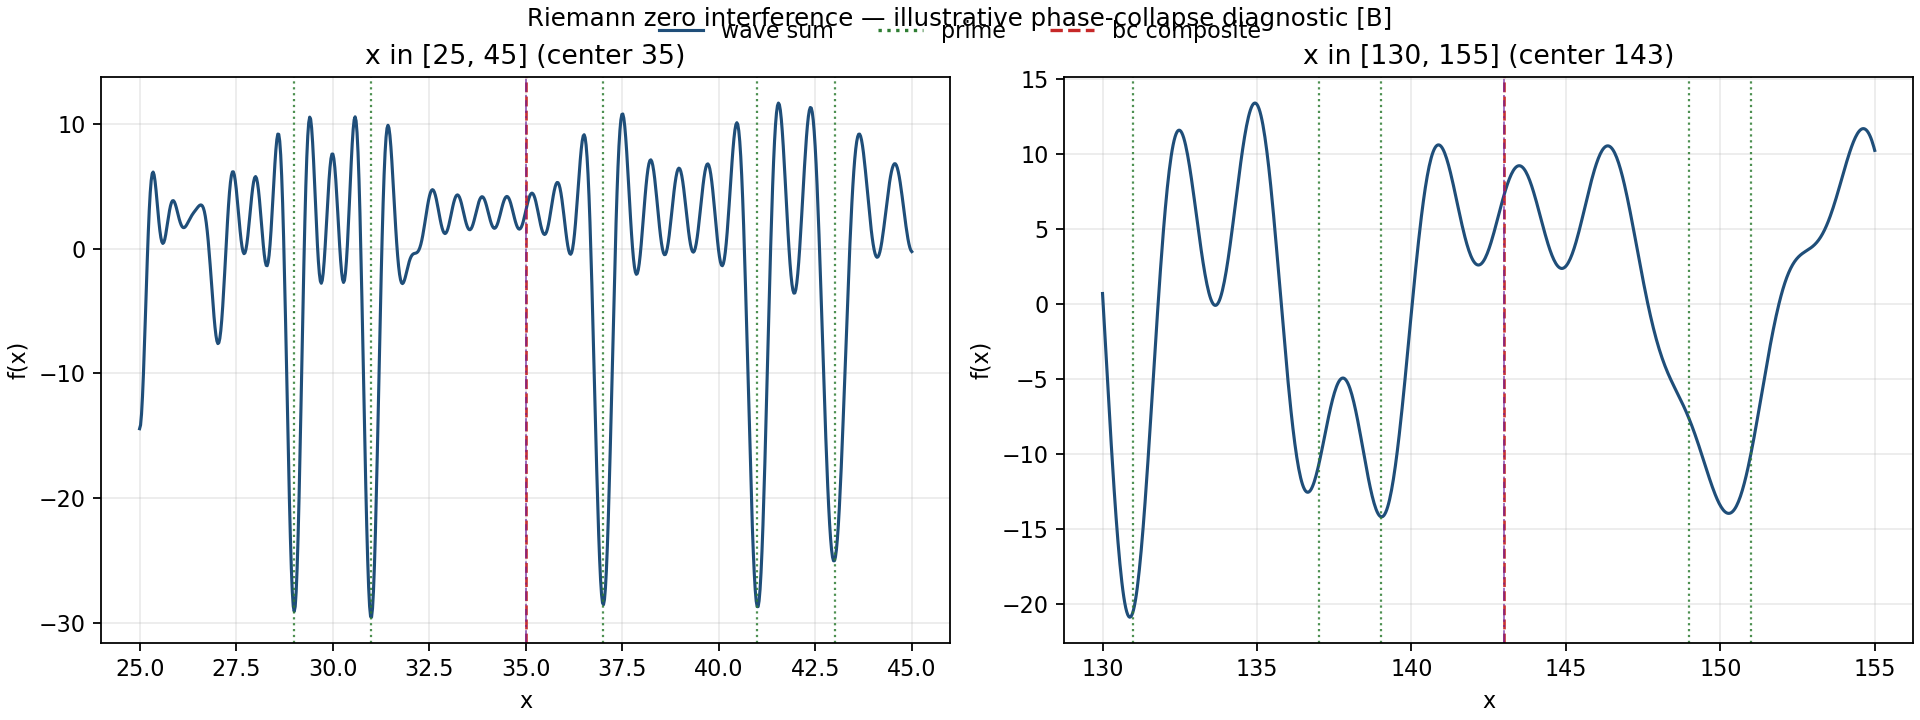
\includegraphics[width=0.85\linewidth]{../exports/riemann_interference_phase_collapse.png}
    \evidence{B} illustrative; E-095.
  \item \textbf{Fig.\,4 --- Fractional-weighted kernel comparison $\alpha{=}0$ vs.\ $\alpha{=}0.5$.}
    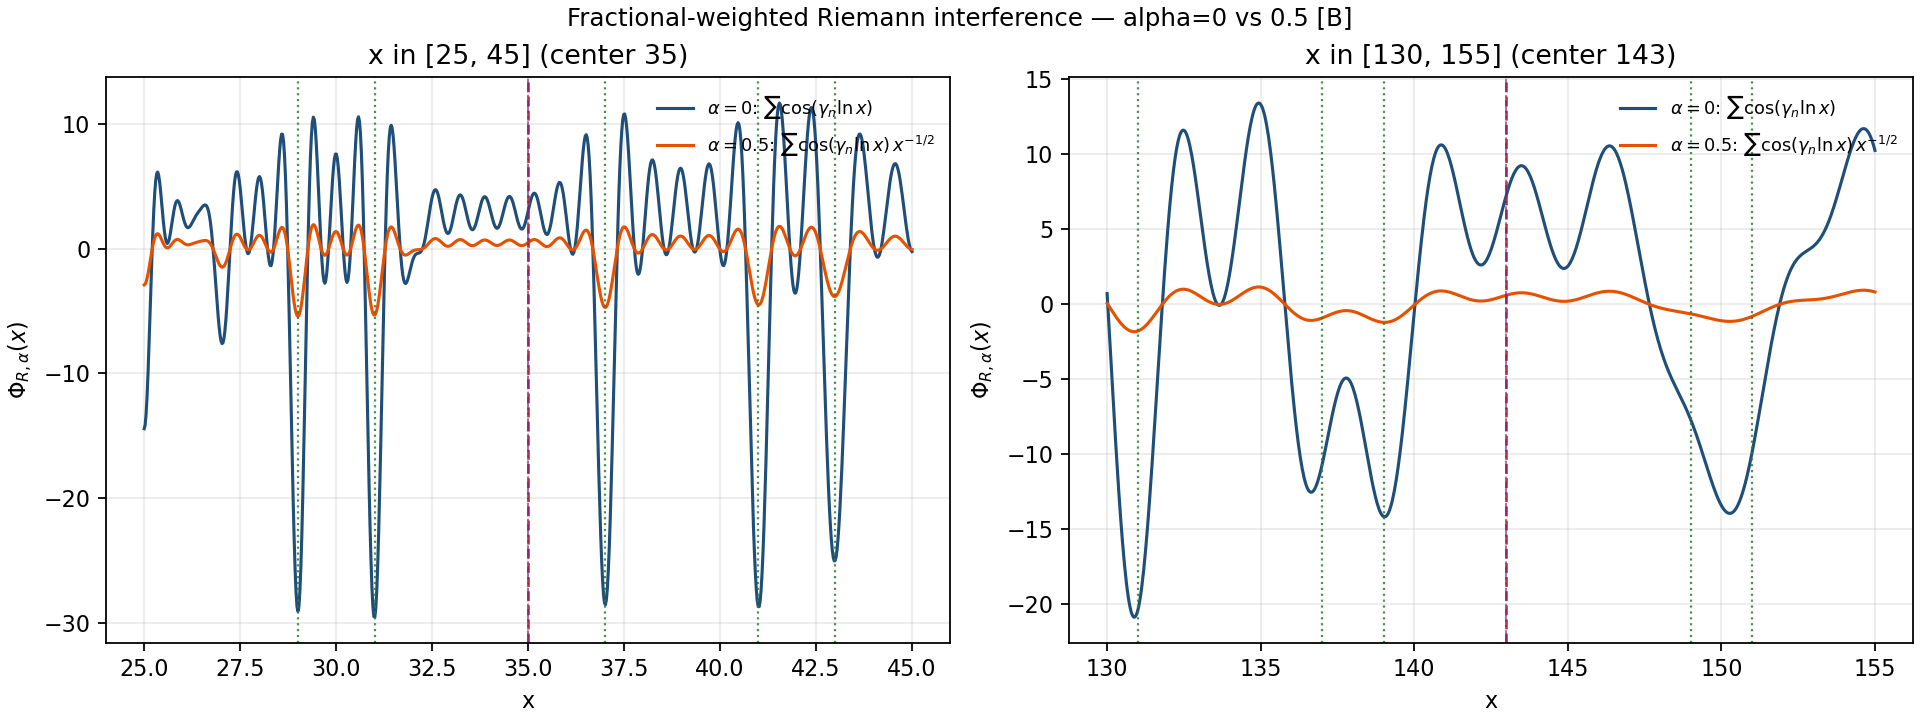
\includegraphics[width=0.85\linewidth]{../exports/riemann_fractional_interference_comparison.png}
    \evidence{B} illustrative; weighted kernel, not Caputo.
  \item \textbf{Fig.\,5 --- Nuclear binding residual $R(A,Z)$ scatter.}
    \placeholder{aus E-092-Export, falls vorhanden.}
  \item \textbf{Fig.\,6 --- Collatz diagnostic atlas panel.}
    \placeholder{Appendix-only; keine Beweis-Interpretation.}
\end{enumerate}

% ===========================================================================
\begin{thebibliography}{99}

\bibitem{Hofbauer2026Energiedoku}
T.~Hofbauer,
\emph{Energiedoku / EABC Renormalization Program},
internal report, 2026.
\placeholder{docs/energiedoku\_exports/eabc\_renormalisierungsprogramm.md}

\bibitem{Hofbauer2026Dumas}
T.~Hofbauer,
\emph{Dumas Cone--Orbit Model},
\repo{docs/theory/dumas_cone_orbit_model.md}, 2026.

\bibitem{Hofbauer2026Riemann}
T.~Hofbauer,
\emph{Riemann Zero Interference Analogy (E-095)},
\repo{docs/theory/riemann_zero_interference_analogy.md}, 2026.

\bibitem{Hofbauer2026Nuclear}
T.~Hofbauer,
\emph{Nuclear Binding Multiscale Analogy (E-092)},
\repo{docs/theory/nuclear_binding_multiscale_analogy.md}, 2026.

\bibitem{OdlyzkoZeros}
A.~Odlyzko,
\emph{Tables of zeros of the Riemann zeta function},
\placeholder{URL / Zitat vervollständigen}.

\bibitem{Bridges2026}
Bridges Conference,
\emph{Mathematics, Art, Music, Architecture, Education, Culture},
2026.
\placeholder{Konferenz-URL und CFP-Referenz.}

\bibitem{Hurwitz1896}
A.~Hurwitz,
\emph{\"Uber die Komposition der quadratischen Formen},
\placeholder{vollständiges BibTeX später}.

\bibitem{Weizsaecker1935}
C.~F.~von Weizs\"acker,
\emph{Zur Theorie der Kernmassen},
\placeholder{vollständiges BibTeX später}.

\end{thebibliography}

\end{document}
